\documentclass[conference]{IEEEtran}
\usepackage{epsfig}
\usepackage{acronym}
\usepackage{amssymb}
\usepackage{amsmath}
\usepackage{amsxtra}
\usepackage{booktabs}
\usepackage{multirow}
\usepackage{url}
\usepackage{fixltx2e}
\usepackage{setspace}
\usepackage{graphicx}

% These define some macro commands I've assembled
\newcommand{\shrink}[1]{{\vspace{-10pt}}}
\newcommand{\comment}[1]{{}}
\newcommand{\forjournal}[1]{{}}
\newcommand{\blind}[1]{{}}
\newcommand{\tout}[1]{{}}
\newcommand{\ol}[1]{{ #1 }}
\newcommand{\omitsection}[1]{{\em Section omitted for blind review process.}}
\newcommand{\omitname}[1]{{\em NameOmitted}}
\newcommand{\etal}{{\em et. al.}}

\begin{document}

\title{ECE 587: Project Report}

% author names and affiliations
% use a multiple column layout for up to three different
% affiliations
\author{
\IEEEauthorblockN{Tanner McWhorter}
\IEEEauthorblockA{Department of Electrical and Computer Engineering\\
Miami University\\
Oxford, Ohio 45056 \\
Email: mcwhortm@miamioh.edu}\\
\and
\IEEEauthorblockN{Isaac Steiger}
\IEEEauthorblockA{Department of Electrical and Computer Engineering\\
Miami University\\
Oxford, Ohio 45056 \\
Email: steigeia@miamioh.edu}

}

\maketitle

%\doublespacing

\begin{abstract}

This paper explores adding axiomatic statements within Non-Axiomatic Reasoning System (NARS), which is an intelligent reasoner that is capable of analyzing incomplete data to develop conclusions and solutions for tasks and questions. This paper further develops OpenNARS, which is an open-source artificial general intelligence (AGI) model that is currently still under development. This project continues the development of OpenNARS to include new features that we believe will be useful when applied to research or industrial products. NARS develops inferences and relationships between its memory structure and the input data in a non-axiomatic manner to reason through a task or question. If the model doesn't have sufficient information to analyze a task, then it will continuously create relationships and inferences, however it may never develop a conclusion. There are many situations when NARS will form "intelligent mistakes" that the user may not want because it will impact the model's overall reasoning ability. Therefore, it would be beneficial to include an axiom token that forces NARS to not make relationships between two objects. This will be useful to ensure that the model doesn't develop obscured relationships that have no real world meaning. Another prominent issue with NARS is that the models require manual setup before they can begin reasoning, which can be troublesome while trying to integrate the model into another project. NARS will be much more integratable by removing and automating the setup parameters that are required to execute a NARS model. The goal of this project was to create a new input copula that will ensure that two components do not form relationships as well as make the NARS GUI more user friendly.

\end{abstract}

\begin{IEEEkeywords} Non-Axiomatic Logic, Reasoner, AGI
\end{IEEEkeywords}

\section{Introduction}

	Non-Axiomatic Reasoning System (NARS) is an open-source artificial general intelligence (AGI) reasoner that is capable of developing conclusions based on incomplete data [1]. NARS hasn't become incredibly popular in the AGI community and we believe that this is due to obvious automation and operation issues. The research presented in this paper hopes to bring light to and fix the issues with the model. The improvements that are mentioned in this paper were developed for the OpenNARS 1.6.5 model because it offers the best graphical user interface (GUI) support, however the code found in [2] does has compile errors. Despite the issues the model may experience, it has been applied to a variety of different tasks. These tasks vary from predicting incoming signal values to playing Super Mario [3]. 
	
	Reasoning systems are models that work with their provided data in order to develop conclusions about a task or question. These conclusions are derived through various techniques such as deduction and induction [4]. Reasoners algebraically manipulate their provided data in order to develop hidden relationships that could derive a conclusion [4]. There are many different types of reasoning mechanisms, however NARS only implements non-axiomatic reasoning. Reasoning systems consist of five main components. The fist component is the formal language that the model uses to receive data and to manipulate the data that it already has stored [5]. The second component is that a reasoner also needs semantics for its formal language in order for the model to understand the meanings of the input data [5]. The third component is that reasoners develop their conclusions through inference rules [5]. These rules allow the model to relate tasks and memories together in an attempt to develop a conclusion. The fourth component is a memory structure that holds the models data and provides the inference rules a work space [5]. The final component that a reasoning system needs is a control mechanism. The control mechanism determines which memories and tasks are associated with various inference rules [5]. This mechanism determines which memories are processed and how they are processed.
	
	Axioms are statements that are assumed to be inherently true and don't need to be questioned [6]. Therefore, non-axiomatic logic refers to logic that does not make the assumption that any of its statements are entirely true. The knowledge that NARS possesses is non-axiomatic and is a summary of NARS' experiences, which can change as new information is presented [1]. Therefore, NARS constantly evaluates the relationships that its formed in its memory structure in order to try and derive new relationships. Each new piece of information that the model is either provided or is discovered through internal reasoning has the potential to alter any of the existing memory nodes. NARS' interrelated memory structures are belief networks that are developed from its entered data by relating objects that have a common attribute between them [7]. 
	
	Narsese is used for the model's input data, which is the formal language for NARS and is used to define object relationships [7]. Narsese is a simple language that defines the relationships between different objects in memory. These relationships contain copulas, which defines the direction and the type of attributes that transfer from one object to another. These copulas consist of inheritance, similarity and many more, which can be found at [8]. With each entered relationship, the model will develop the entered belief nodes and then it develops relationships between these new nodes and any existing memory structures that are within the object's scope. We defined an object's scope as the nodes that the object can develop relationships given the different copulas between the nodes. NARS can run into issues where the model will develop impractical real-world relationships that the user may not want, which was mentioned by Pei Wang to be an issue with the design of the model [5]. This is due to the fact that NARS will develop a relationship link between two nodes if there is a common node or relationship link between them. If a model develops an undesired relationship, then it will impact the model's reasoning for a given situation. This is why we developed a new input token to define objects that are not related to one another.
	
	When the OpenNARS GUI is first launched, it brings the user to a title menu where they can choose between the OpenNARS model and various other applications of OpenNARS, such as pong. The user has to select OpenNARS from this menu screen before they begin interacting with a NARS model. Once the user is within the OpenNARS interface, they then need to specify various run-time parameters, such as processing speed and the amount of information that is displayed through the GUI. The user also has to specify which Narsese memory file they would like to load in. If a user wanted to integrate a reasoner into another project, then these setup steps would be a real drawback for using this model. Therefore, it will be very useful to automate the OpenNARS GUI to launch straight to the NARS interface and have these settings and memory file already defined. These additions will hopefully make this model more accessible for researchers to work with. 	
	
	This paper is organized as follows. Section II explains the NARS model with more details and Section III describes our methods for improving the NARS model with our new token. The experimental setup and results are then discussed in Section IV. The paper then finishes with our conclusions and future ideas about the project in Section V.
	
	
\section{Background}
	NARS was developed by Pei Wang for his dissertation in the 90's [5]. This model was defined as a theory, and had very little implementation. There are various NARS projects that have started since the release of his dissertation, however they each have their own issues. The major contribution of his research was the push to model general intelligence towards non-axiomatic logic using various reasoning and inference rules, as well as defining the formal language that NARS uses [5]. The model that he defined would be able to able to learn from entered data in order to make conclusions.

	NARS' CAD flow is shown in Figure 1. Data moves from one stage to another based on the NARS cycle. The speed of the NARS cycle is defined by the user in the NARS GUI. A NARS cycle is the change from one state to another that NARS' data goes through. These states are labeled with numbers in Figure 1. The Narsese input data is entered into the model and gets held in a buffer, where it waits until it is selected to move to the memory, which is based on a priority function [1]. It's important to note that all of the inputs that are in an input file will be pushed to the buffer at the same time. The inputs are represented as relationships in the buffer as they were defined in the input file. This buffer plays a pivotal role for conducting non-axiomatic logic, which will be explained later on.

	 \begin{figure}[ht!]
\centering
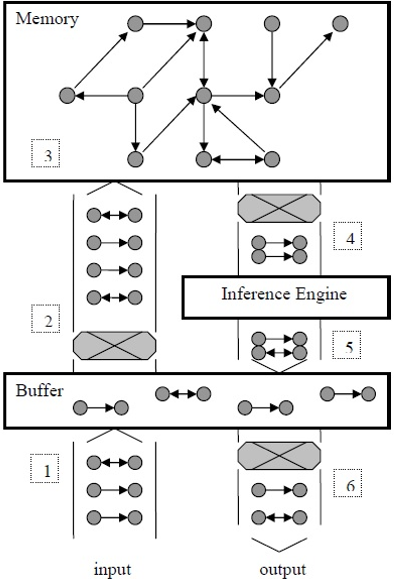
\includegraphics[width=80mm]{Picture1.png}
\caption{NARS Data Flow [1] \label{overflow}}
\end{figure}
	
	 Once the entered relationship moves to the memory, the model then develops relationships with these new nodes and the previously existing memory structure [1]. The relationships that are developed are based on the scope of an object and the different types of relationships that are within that scope. These relationships are called term links inside of NARS' concept network. The concept network is what NARS defines it's memory structure as. Because the model is non-axiomatic, it will constantly try to derive new relationships between the different belief nodes. The memory structure uses a priority level system that determines how much processing time a certain belief will obtain during a given NARS cycle [9]. The priority level for each node changes at each NARS cycle. The priority level for a task can drop so low that the task is no longer considered. This guarantees that NARS will never get stuck trying to evaluate an impossible task [9].
	 
	 At each NARS cycle, a task and a belief node are passed from the memory to the inference engine to try and reason through the task or question [1]. This inference engine consists of various non-axiomatic logic (NAL) layers. Each layer implements a different type of logic (inductive, probabilistic, fuzzy, etc) in order to discover hidden relationships that may be present [1]. Searching for these hidden relationships allows the model to reason through data and develop conclusions. If the inference engine was unable to develop a solution or conclusion for the task or question, but it was able to develop an intermediate hidden relationship between the task and memory, then these new relationships are passed to the buffer. At the next NARS cycle, these new memories are sent back to the memory, where they develop relationships with the current memory structure. This cycle of developing hidden relationships and incorporating these hidden relationships into the existing model allows NARS to develop very complicated memory structures. The buffer plays a pivotal role that allows the model to learn from the conclusions that it derives. If the model is able to develop a conclusion for the task, then the solution is passed to the buffer, where it gets pushed to the output and displayed through the GUI. 
	 
	 A very interesting aspect of NARS is that if it is unable to develop a conclusion, then it will constantly evaluate its memories in an attempt to solve the task [1]. If an infinite loop like this occurs, then the model will never display a conclusion to the GUI. It will simply continuously evaluate each of its belief nodes. Even if there are no new possible connections to be made, the model will still evaluate each of its relationships. This is a fundamental aspect of non-axiomatic reasoning. Another interesting aspect of NARS is that it develops conclusions that are not based entirely on computation, but a mixture of computation and previous experiences [9].
	 
	Pei Wang identified three issues with the overall design of NARS.   	 
	 
\begin{enumerate}
  \item The first issue is derived from the fundamental nature of NARS. Because NARS implements non-axiomatic reasoning, the model does not support axiom relationships such as consistency and completeness because the terms would constantly be subject to changed when new information is presented [5].
  \item The second downside that was mentioned is that NARS will never be able to develop human-level intelligence because the reasoning mechanisms between the two are so different [5]. The human mind is very complex and it shouldn't be surprising that a computer simulation is unable to achieve human-level reasoning. While NARS may not be able to develop human-level reasoning, it is able to conduct reasoning in an intelligent manner [5].
  \item  NARS is an AGI model, which means it can be applied to any problem and it will do its best to develop a conclusion using the data that it's been provided. While this may seem like an advantage, Pei Wang actually mentions it as being a downside of the model. Because NARS was not designed to solve any particular task, the model runs into issues where it develops "intelligent mistakes", which is the third flaw of the design [5]. These mistakes make sense for NARS because it was able to develop a relationship between the two beliefs, however this relationship may have no real-world meaning.
\end{enumerate}	 
	 
	 Figure 2 contains Narsese inputs and outputs of an "intelligent mistake" that was described by Pei Wang. The first line states that an apple is a fruit with a 100\% frequency value and a 90\% confidence value. The frequency corresponds to the amount of positive evidence to the total evidence and the confidence value is the likelihood that the conclusion will change [7]. A higher confidence value corresponds to a more stable conclusion, while a higher frequency value has more supportive evidence. Apples and pineapples are then provided a color description. The fourth line of Figure 2 states that a pineapple is a fruit and the following line asks if a pineapple is an apple. The conclusion that NARS develops is the "Answer" line in Figure 2. For the information that the model was provided, it developed the conclusion that yes a pineapple is an Apple, but with a confidence level of .45 and a frequency of 1. The concept network that NARS develops for this example is shown in Figure 3. This is simply a screen shot of NARS' memory when it provided its conclusion. This memory would have grow much larger if it were to run longer because it would continuously make relationship nodes in order to develop an more accurate solution to the task.
	 
\begin{figure}[ht!]
\centering
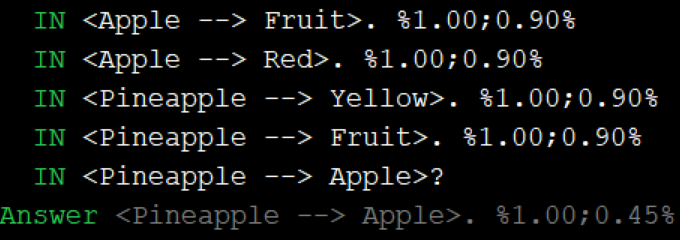
\includegraphics[width=90mm]{Incorrect.png}
\caption{Results of the Fruit Example \label{overflow}}
\end{figure}

\begin{figure}[ht!]
\centering
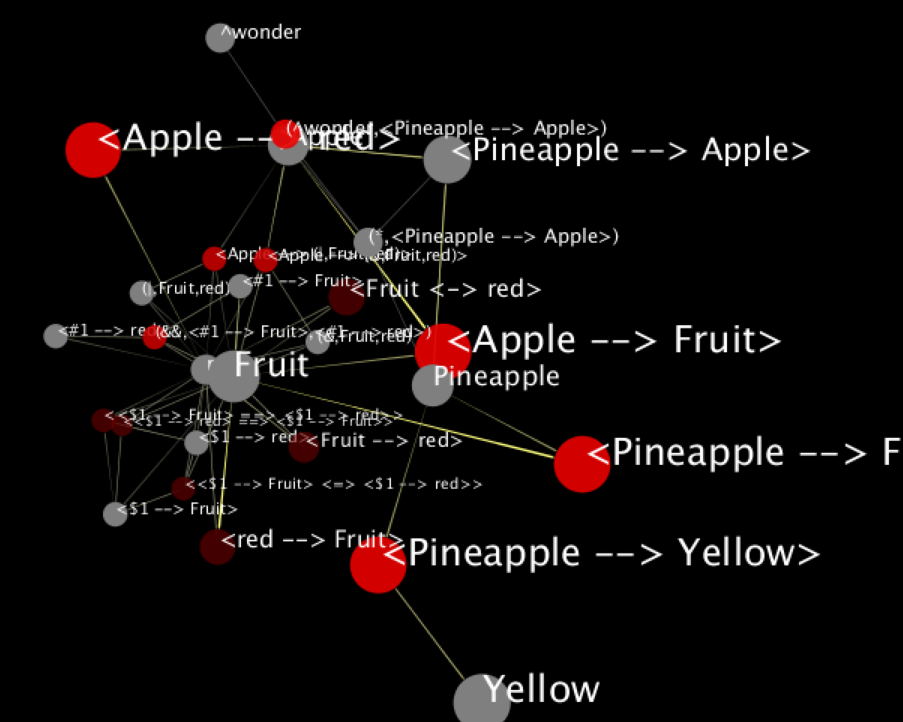
\includegraphics[width=90mm]{Memory.png}
\caption{Concept Network of the Fruit Example \label{overflow}}
\end{figure}


\section{Not-Equals Token}
	The goal of the not-equals token is to define two objects that are not related at all. There are instances when its beneficial to have axioms that excludes the possibility of an "intelligent mistake". In the previously explained example, it would have been beneficial to have a token to state that a pineapple is not an apple. Including this token goes against the non-axiomatic logic that NARS uses, therefore it needed to be implemented in a careful manner. We determined that the most efficient method for implementing this was to force NARS to not make relationships between two objects that are defined using a not-equals token. This method has the downside that NARS will constantly try to develop a relationship between the objects if there is sufficient data to justify such a connection, however the connection is blocked by the not-equals token. Figure 4 depicts the desired results for this token. If NARS is unable to draw a conclusion for a task or question, then it will continuously evaluate the task or question until there is sufficient information to make a conclusion. Therefore, our resulting model will simply continuously make inferences when its asked if a pineapple is an apple because it will be unable to draw relationships between the two objects.  	
	
\begin{figure}[ht!]
\centering
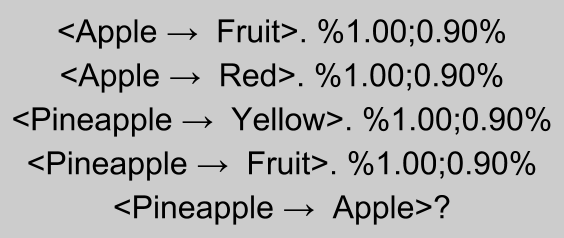
\includegraphics[width=90mm]{Desired.png}
\caption{Desired Results of the Fruit Example \label{overflow}}
\end{figure}	

	With the general approach of blocking unwanted relationships, we discovered that there were two different paths that this could be implemented through. The first option would have been to use NARS operations. NARS has various operations defined that were used for the example applications in [3]. These operations consisted of moving a certain direction, flipping switches and other various actions that could be useful if the model was ever implemented in a product. The idea was to include an operation that stated that two objects are unrelated, however this direction would have required major changes throughout the CAD flow. The operation token was included very easily, however accessing the specific beliefs that were being evaluated in the memory would have been difficult to access. Therefore, we did not peruse this path.
	
	The second option was to develop a new Narsese copula to define objects that aren't the same. This required us to declare the new copula within the Narsese language as well as implementing the not-equals logic throughout NARS' memory structure and inference engine. This route was slightly easier than the previously discussed method because we could base our changes off of the existing input copulas. Whenever the not-equals input copula is called, the associated objects are added to a list. As the memory develops relationships with its various belief nodes, it checks to ensure that they haven't been defined with the not-equals token. If they have been defined with the not-equals token, then the model will reject that relationship and NARS will continue onto the next set of beliefs to be processed. As long as the user enters the not-equals token before entering the rest of the memory, NARS will not develop any relationships between the objects. It will constantly try to, however it will be unable to complete them. The not-equals Narsese copula is defined as "!->".

		
\section{Results}	
	In this section we discuss the accomplishments of the paper. First, we explain the errors that were causing the model to not compile. Second, we explain the additions that we've made to the GUI in order to make it more user-friendly. Finally, we explain the experimental setup and we measure and discuss the impact that our new Narsese copula has on NARS' reasoning process. We measured the effects that our new copula had on NARS' reasoning by measuring the frequency and confidence values of the conclusions that it derives. The resulting model can be found at [10].

\subsection{Compile Issues Correction}
	Since OpenNARS is an open-source project and is still underdevelopment, it makes sense that there's errors in the model. OpenNARS is currently in its third version of development, however there is still interest in the older version models because of their simplicity. The newer version of OpenNARS requires Maven dependencies, which adds to the complexity of a project if a researcher wanted to integrate OpenNARS into an existing project [11]. Since OpenNARS 1.6.5 only requires Java, it is much easier to integrate into other projects. The compile issues consisted of classes being in the wrong directory. The developers moved these files to separate folders while they were trying to implement additional NAL layers, however the implementation for these new layers was never completed. Therefore, moving the working classes back to their home directory fixed the compile errors that were experienced with the OpenNARS 1.6.5 model.

\subsection{User-Friendly Additions}
	When the user launches the NARS GUI, it now opens to the interactive NARS window with the NARS model automatically running. The processing speed is set to maximum and the amount of information that is displayed to the screen is set to minimum. Setting the amount of displayed information to the minimum allows the user to only see the entered data and NARS' conclusions, if it were to develop any. It was determined that the intermediate relationships aren't very important when the user is using NARS as a reasoner. As the GUI launches, it also loads in a Narsese memory file that is defined by the user. The user can define this file by providing the file path in an index file. The model automatically begins developing relationships for the provided memory file as the GUI is launched, which allows a user to execute their models through a command line. This was previously not possible. If the user wants to define a NARS model through the GUI and not through a separate Narsese file, then they can simply define a memory in the index file that is blank and they can enter the relationships once the GUI has launched.
	
	It should be noted that the user needs to include a large delay, around 10,000,000, as the first Narsese input if they would like to see the first few inputs appear in the GUI window. The memory will still load, however it won't be displayed to the user. The concept network will contain the memories. This is required because there is a delay between the GUI window popping up and when NARS is first provided its memory. The GUI is launched the same time the model is provided a memory, however the window doesn't appear fast enough for the user to observe the first few inputs.    

\subsection{Experimental Setup}
	The model was tested using various Narsese memories that consisted of a wide range of node scopes. The experiments were broken down into three parts. The first part consisted of conducting fundamental tests to determine if the not-equals token logic was being implemented correctly or not. The second part conducts experiments to determine how our token impacted NARS' overall reasoning in terms of confidence and frequency values. It is hard to identify a concrete basis for measurement because NARS can be unpredictable at times. A major difficulty with these tests is that different machines may develop different results due to their processing capabilities. We wanted to demonstrate the impact of our new not-equals token, so we developed a string of benchmarks that grew with node scope, which can be seen in Figure 5. It should be noted that the benchmarks that are marked with a * have additional copulas that the others did not contain. The number of copulas determines the scope of the benchmark. In order to accurately measure the impact that our token had on the non-axiomatic logic, we increased the scope of a question and compared the conclusion's confidence and frequency values of the benchmark memories with an intermediate node "turned on" and "turned off". Turned off and on simply refer to whether or not the two primary nodes have the not-equals token between them. Turned on refers to a memory that didn't use our token and turned off refers to a memory that did use our token. With each successive benchmark, the scope of the question grew. The scope of the question refers to the number of defined relationships that are between the nodes that are under question. We wanted to include many of the same input copulas for this test to ensure that the change in confidence and frequency was due to our new token and not from the different properties that the different input copulas have. The third experiment reproduced the pattern classification technique that was proposed by [12]. This example is intended to prove that our token can handle higher order relationships.
	
	Each of the benchmarks that were used were analyzed by NARS for the same period of time to allow for comparable results. Since NARS models may develop more confident answers with more processing time, we needed to test each benchmark using the same amount of processing time. If it takes a model longer to develop a conclusion, then the results wouldn't be comparable unless each of the benchmarks were processed for the same amount of time. Therefore, each benchmark was processed for 10,000 NARS cycles. Through our experiments, this time was typical for a memory to become relatively stable. We are referring a stable memory as a memory that is not making large conclusions with the data that it contains.

\begin{figure}[ht!]
\centering
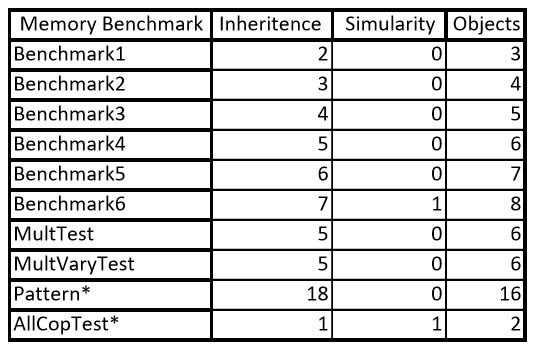
\includegraphics[width=90mm]{BenchmarkTable.png}
\caption{Description of Benchmarks \label{overflow}}
\end{figure}	

\subsection{Simple Tests}
	A very simple test was conducted to determine if the not-equals token was working properly. We wanted this test to be as small as possible to observe how our token impacted NARS' memory. The input memory that was used consisted of inheritance links between Tanner, Isaac and Human, which can be seen in Figure 6. The resulting concept network is shown in Figure 7. The model was stopped after the same number of cycles as was previously explained in order to prevent the memory from becoming too large to evaluate. Our not-equals token can be seen in the concept network and it is linked between Tanner and Isaac. This relationship identifies that the model will not make connections between these objects. When the model is asked whether or not Tanner is Isaac, the task is rendered invalid at the buffer because there is no possible way that the two objects are the same due to our copula. The other nodes are trying to draw a relationship between Tanner and Isaac, however the model is not able to because of our token. While this may be a simple test, it shows that our token forces the model to not make connections between the objects.

\begin{figure}[ht!]
\centering
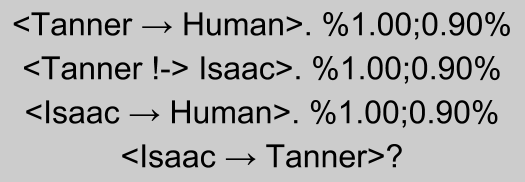
\includegraphics[width=90mm]{SimpleTest.png}
\caption{Simple Test Memory \label{overflow}}
\end{figure}	

\begin{figure}[ht!]
\centering
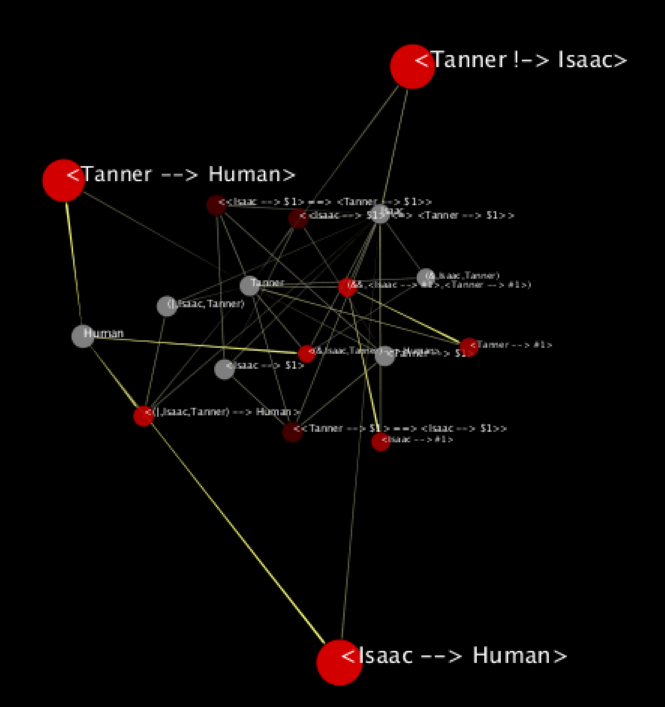
\includegraphics[width=90mm]{SmallTest.png}
\caption{Simple Test Concept Network \label{overflow}}
\end{figure}	

	Our token was then tested to determine if the not-equals token worked for multiple instances of not-equals in a memory. This was tested by providing NARS a memory that had many not-equals token and then asking the model if the objects were related. Each of the questions were conducted under inheritance. This test is the benchmark named MultTest. The model was unable to develop any conclusions, which supports the notion that our not-equals copula works for multiple instances of it in a memory.
	
	We then needed to determine if our token was applicable towards Narsese copulas other than inheritance. Similarity was then tested because it is similar to  inheritance. The same test that was previously explained was conducted using similarity instead of inheritance questions. This test is the MultVaryTest benchmark. Our not-equals token prevented the model from developing any relationships that could answer the tasks, which supports that our token works for similarity copulas as well.

	The not-equals copula was then tested against every one of the possible Narsese copulas in order to ensure that the not-equals token was rejecting relationships between every other type of relationship. The AllCopTest benchmark tested our not-equal token against every Narsese copula. The memory is similar to the previous example, however it continues to ask the model if Tanner and Isaac are related through any of the other copulas. The model was unable to develop a conclusion for this memory, which suggests that our token works against developing relationships between every possible method that relationships can be formed through. It would be reasonable to assume that since the not-equals token blocks the relationships between all of the copulas, that the not-equals token works across NARS' memory as a whole. This is supported by the fact that NARS uses these Narsese copulas to develop its memory structure. This further supports the case that our not-equals token is working properly.
	
	Each of these tests further supports that our not equals token works properly. It should be noted that in order for NARS to not have an undesired relationship in its memory, the not-equals token needs to be called before both of the objects have been provided to NARS. Our token does not retroactively remove connections that have been made in the memory, however it will prevent the model from being asked questions about these objects if this were to ever happen. The questions are thrown as invalid when they are entered because the not-equals axiom is within the buffer, which states that these connections are not possible. Each relationship is held in the buffer before being passed to the memory, which is why it is beneficial to remove the question before it makes it to the memory. It should also be noted that the benchmarks had to be tested in separate files because the not-equals token would interfere with the base cases. Base cases refer to the benchmarks that did not use our copula. When a memory is loaded into NARS, all of the input relationships are held in the buffer, which will recognize that the not-equals token is present. When this happens, the questions and relationships that are related to the objects defined with a not-equals token in the base case memory are removed. This happens even when there is a reset in-between the test case and base case because when a memory is loaded, all of the inputs are pushed to the buffer at the same time. Our model clears the not equals list when reset is called, however if the base cases are in the same memory file as the test cases, then the model will block the relationships in the base case as well. It is reasonable for NARS to declare a question invalid because if it didn't, then it would possibly get stuck trying to analyze an impossible task. 
	
\subsection{Comparison of Confidence and Frequency Values When Using Not-Equals Token}
	Once it was determined that the not-equals copula was working properly, we then conducted tests to determine how our copula impacted NARS' reasoning. This was required to demonstrate that our method was not simply preventing the user from asking questions about objects that were declared with the not-equals token, but that it was actually blocking relationship paths within NARS' memory. The impact that our token had on a model was measured by comparing the confidence and frequency values of a conclusion that NARS would draw for a memory that had or not-equals token and one that didn't have our not-equals token. The confidence value results are shown in Figure 8. Benchmarks 1-6 were used to collect this data. The blue line is the tests that were conducted with a node turned off (ie. using our not-equals token) and the orange line is the tests that were conducted with the node turned on (ie. not using our not-equals token). The first benchmark was a test that was similar to the first simple test, which is why the model was unable to develop a conclusion. As the scope increases for the node under question, the model tends to develop higher confidence values, however it is consistently below the test points that were collected without our token. The scope of a node under question refers to the number of relationships between the two nodes under question. The frequency results are shown in Figure 9. The frequency value of the turned off tests had a higher frequency for 5 and 6 nodes in the scope, which is believed to be due to a lack of total evidence that the model had to base its conclusion on. This supports the fact that our token was able to successfully block relationships that would have otherwise produced negative evidence. The base case had a lower frequency because the intermediate node had negative evidence for the conclusion. It should be noted that at these nodes in scope, the confidence value is much lower than the previous tests. This signifies that while the model had more positive evidence versus evidence as a whole for these cases, the model was much less confident in its conclusion. This lower confidence is due to the memory not having as many relationship connections to support the conclusion. The confidence value increased at 8 nodes in the scope as the frequency of the conclusion drops, which signifies that there was negative evidence presented. This negative evidence was due to our token stating that an intermediate node was not the same as another.
	
\begin{figure}[ht!]
\centering
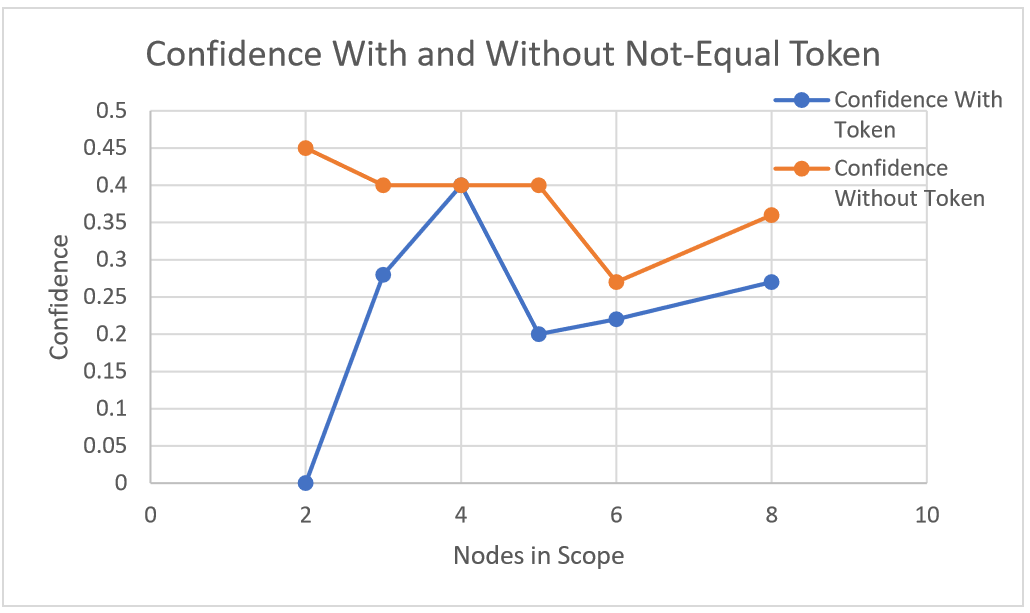
\includegraphics[width=90mm]{Confidence.png}
\caption{Confidence of Conclusions \label{overflow}}
\end{figure}	

\begin{figure}[ht!]
\centering
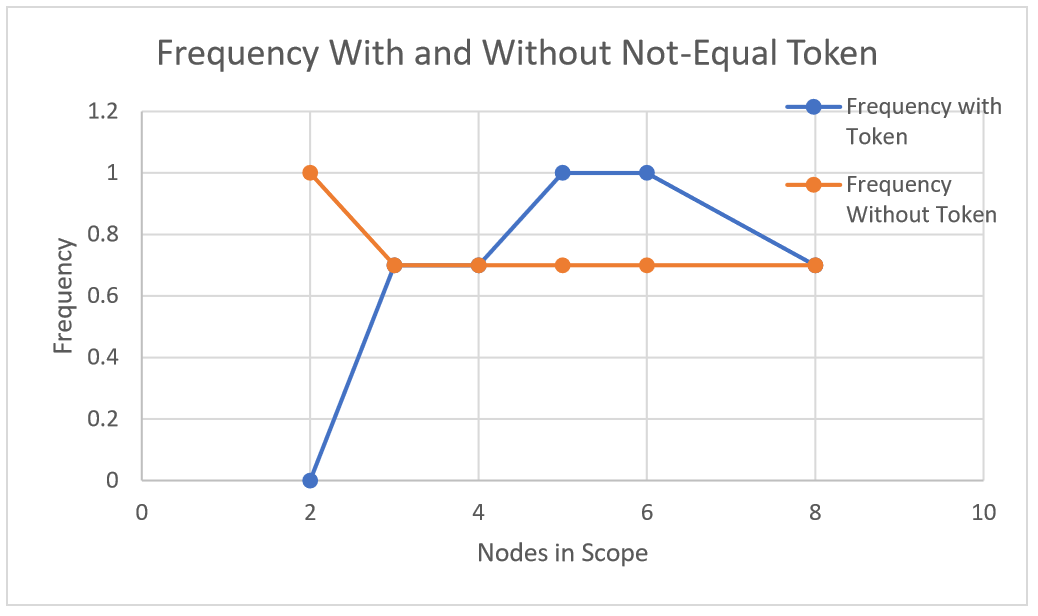
\includegraphics[width=90mm]{Frequency.png}
\caption{Frequency of Conclusions \label{overflow}}
\end{figure}	
	
	 It should be noted that the frequency and confidence results for the node being on and off were the same for 4 nodes in the scope. This is likely due to the benchmark developing more meaningful intermediate relationships, which increased the confidence values for our not equals test. It should also be noted that because NARS is non-deterministic with how it develops conclusions, we tested each of these benchmarks ten times. Surprisingly, it produced the same results with each iteration, which is why the results are not presented as an average. This may not be the case on other machines.

\subsection{Pattern Recognition}
	We then tested our not-equals token to determine how it handled variables in a memory structure. This increases the testing depth because these variables act as hidden relationships until they are sent to the memory. This test was conducted using the Pattern benchmark, which was designed based on the pattern recognition technique that was proposed by Pei Wang's graduate student in [12]. The benchmark consisted of two signals that each had the exact same frequency sequence, but defined separately. One signal was defined as an FM signal and the other was defined as an AM signal. These patterns were short, however they still demonstrated how input variables are used. Figure 10 depicts the results of using our not-equals token and Figure 11 depicts the results of not using our not-equals token. The test conducted using our token was unable to develop a conclusion, while the test not using our token was able to develop a conclusion. While the confidence of the answer in Figure 11 is low, it is still promising to observe that our token was able to prevent relationships between variables.
	
\begin{figure}[ht!]
\centering
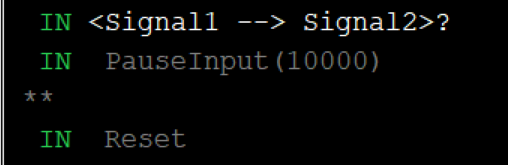
\includegraphics[width=90mm]{PatW.png}
\caption{Pattern Test with Not-Equals \label{overflow}}
\end{figure}	

\begin{figure}[ht!]
\centering
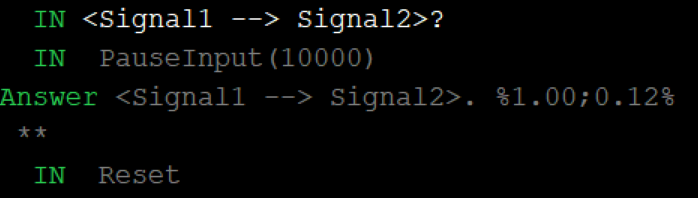
\includegraphics[width=90mm]{PatWo.png}
\caption{Pattern Test without Not-Equals \label{overflow}}
\end{figure}	
	

\section{Conclusions and Future Ideas}

	Our testing and comparisons strongly suggests that our not-equals token works as we had desired. Not only was it able to prevent relationships from being formed between objects, it also had measurable impacts on NARS' overall reasoning. If our token had no effect on the confidence and frequency results of a conclusion, then it may have been speculated that our token was simply blocking the user from asking the model questions about nodes that were defined with our token. The results support that our token did indeed alter the way that NARS conducts reasoning. 
	
	We hope that the work explained in this paper will allow OpenNARS to be more accessible for researchers to integrate into existing projects. Automating NARS allows a user to execute the GUI from the command line and the model will automatically begin reasoning through a memory. While setting the default processing speed to maximum has the downside of requiring the user to include a delay as the first input, the model still develops the same relationship as it would if it were processing at a slower speed. Defaulting to the fastest speed will allow a user's model to develop a stable memory in an efficient time frame that is hopefully reasonable enough to integrate it into projects that could benefit from a general reasoner. The volume of data that is shown through the GUI is set to zero to only display the user's inputs and the model's conclusions, which will prevent users from getting overwhelmed by the complexity of NARS' memory structures. 

	It should be noted that this model had many bugs in the original version that unfortunately followed over into this project. For example, there are instances when you provide the model an empty file in order to manually provide the model inputs, however if the user waits too long, then the first input they enter will be ignored by the model. There are instances of this in the original model if you provide the model many inputs at once when it is running at full speed, which this model is running at as well.

	Future improvement for this model would be to have the model write its conclusions to a text file. This would allow researchers to use NARS' results for another program by simply parsing the outputted text file. This could be relatively easily integrated into the model by looking for where the model emits its memory to the GUI. There is a function that NARS uses to display its conclusions through the GUI (memory.emit()). A researcher could print the memory element that is emitted during that function call to a text file in order to accomplish this. 
	
	It would also be beneficial to remove the confidence and frequency values that get associated with the not-equals token in the GUI. These parameters are displayed as the default values when this token is entered, however they have no impact on how the model uses the relationship.

\section{References}
[1] Pei Wang, “A Logical Model of Intelligence – An Introduction to NARS,” \url{https://sites.google.com/site/narswang/home/nars-introduction}

[2] Hammer, Patrick. “NARS - Downloads.” Google Drive, Google, 19 Feb. 2017, \url{drive.google.com/drive/folders/0B8Z4Yige07tBUk5LSUtxSGY0eVk}

[3] Wang, Pei. “Opennars Application Programs.” GitHub, 29 Apr. 2015, \url{github.com/opennars/opennars/wiki/Application-Programs}

[4] “AI Is about Machine Reasoning – Or When Machine Learning Is Just a Fancy Plugin.” Reasoning.World, 23 May 2017, \url{www.reasoning.world/ai-is-about-machine-reasoning}
\url{-or-when-machine-learning-is-just-a-fancy-plugin/}

[5] Wang, Pei, 1996, Non-Axiomatic Reasoning System - Exploring the Essence of Intelligence, \url{https://www.researchgate.net/publication/2690739_Non-Axiomatic_Reasoning_System_-_Exploring_the_Essence_of_Intelligence}

[6] Brown, Robert G. What's an Axiom. Duke University, 17 Dec. 2007, \url{webhome.phy.duke.edu/~rgb/Philosophy/axioms/axioms/node27.html}

[7] Wang, Pei. “From NARS to a Thinking Machine.” Temple University College of Science and Technology, Temple University, \url{cis.temple.edu/~wangp/Publication/roadmap.pdf}

[8] “OpenNARS Input Output Format .” GitHub, 14 Aug. 2018, \url{github.com/opennars/opennars/wiki/Input-Output-Format}

[9] Wang, Pei. “Computation and Intelligence in Problem Solving.” Temple University Department of Computer and Information Sciences , \url{pdfs.semanticscholar.org/1330/5ce22a59ca18f0f56ab8de13af074a167197.pdf}

[10] Steiger, Isaac. “ECE587.” GitHub, 4 Dec. 2018, \url{github.com/steigeia/ECE587}

[11] “Opennars/Opennars.” GitHub, 24 Oct. 2018, \url{github.com/opennars/opennars}

[12] Zaikowski, Matthew. “Pattern Recognition In NARS.” College of Science and Technology, Temple University, 4 Apr. 2011, \url{www.cis.temple.edu/~pwang/Implementation/Cases/MatthewZaikowski.doc}

\end{document}
